

%%%%%%%%%%%%%%%%%%%%%%%%%%%%%%%%%%%%%%%%%12pt: grandezza carattere
                                        %a4paper: formato a4
                                        %openright: apre i capitoli a destra
                                        %twoside: serve per fare un
                                        %   documento fronteretro
                                        %report: stile tesi (oppure book)
\documentclass[14pt,a4paper,openright,twoside]{extreport}
%
%%%%%%%%%%%%%%%%%%%%%%%%%%%%%%%%%%%%%%%%%libreria per scrivere in italiano
\usepackage[italian]{babel}
%
%%%%%%%%%%%%%%%%%%%%%%%%%%%%%%%%%%%%%%%%%libreria per accettare i caratteri
                                        %   digitati da tastiera come � �
                                        %   si pu� usare anche
                                        %   \usepackage[T1]{fontenc}
                                        %   per� con questa libreria
                                        %   il tempo di compilazione
                                        %   aumenta
\usepackage{newlfont}
\textwidth=450pt\oddsidemargin=0pt

\usepackage[latin1]{inputenc}
%%\usepackage[utf8]{inputenc}

%
%%%%%%%%%%%%%%%%%%%%%%%%%%%%%%%%%%%%%%%%%libreria per impostare il documento
\usepackage{fancyhdr}
%
%%%%%%%%%%%%%%%%%%%%%%%%%%%%%%%%%%%%%%%%%libreria per avere l'indentazione
%%%%%%%%%%%%%%%%%%%%%%%%%%%%%%%%%%%%%%%%%   all'inizio dei capitoli, ...
\usepackage{indentfirst}
%
%%%%%%%%%libreria per mostrare le etichette
%\usepackage{showkeys}
%
%%%%%%%%%%%%%%%%%%%%%%%%%%%%%%%%%%%%%%%%%libreria per inserire grafici
\usepackage{graphicx}
%
%%%%%%%%%%%%%%%%%%%%%%%%%%%%%%%%%%%%%%%%%libreria per utilizzare font
                                        %   particolari ad esempio
                                        %   \textsc{}
\graphicspath{{image/}}
\usepackage{newlfont}
%
%%%%%%%%%%%%%%%%%%%%%%%%%%%%%%%%%%%%%%%%%librerie matematiche
\usepackage{amssymb}
\usepackage{amsmath}
\usepackage{latexsym}
\usepackage{amsthm}
%\usepackage[breaklinks=true]{hyperref}
\usepackage[hyphens]{url}

%
\oddsidemargin=10pt \evensidemargin=20pt%impostano i margini
\hyphenation{sil-la-ba-zio-ne pa-ren-te-si}%serve per la sillabazione: tra parentesi
					   %vanno inserite come nell'esempio le parole
%					   %che latex non riesce a tagliare nel modo giusto andando a capo.

%
%%%%%%%%%%%%%%%%%%%%%%%%%%%%%%%%%%%%%%%%%comandi per l'impostazione
                                        %   della pagina, vedi il manuale
                                        %   della libreria fancyhdr
                                        %   per ulteriori delucidazioni
\pagestyle{fancy}\addtolength{\headwidth}{20pt}
\renewcommand{\chaptermark}[1]{\markboth{\thechapter.\ #1}{}}
\renewcommand{\sectionmark}[1]{\markright{\thesection \ #1}{}}
\rhead[\fancyplain{}{\bfseries\leftmark}]{\fancyplain{}{\bfseries\thepage}}
\cfoot{}
%%%%%%%%%%%%%%%%%%%%%%%%%%%%%%%%%%%%%%%%%
\linespread{1.3}                        %comando per impostare l'interlinea
%%%%%%%%%%%%%%%%%%%%%%%%%%%%%%%%%%%%%%%%%definisce nuovi comandi
%
\begin{document}

\begin{titlepage}
\begin{center}
{{\Large{\textsc{Alma Mater Studiorum $\cdot$ Universit\`a di
Bologna}}}} \rule[0.1cm]{15.8cm}{0.1mm}
\rule[0.5cm]{15.8cm}{0.6mm}
{\small{\bf SCUOLA DI SCIENZE\\
Corso di Laurea in Informatica }}
\end{center}
\vspace{15mm}
\begin{center}
{\LARGE{\bf VsnLib:}}\\
\vspace{3mm}
{\LARGE{\bf una interfaccia unica di configurazione}}\\
{\LARGE{\bf per stack di rete virtuali tramite pacchetti netlink}}\\
\end{center}
\vspace{40mm}
\par
\noindent
\begin{minipage}[t]{0.47\textwidth}
{\large{\bf Relatore:\\
Chiar.mo Prof.\\
Renzo Davoli}}
\end{minipage}
\hfill
\begin{minipage}[t]{0.47\textwidth}\raggedleft
{\large{\bf Presentata da:\\
Simone Preite}}
\end{minipage}
\vspace{20mm}
\begin{center}
{\large{\bf Sessione di Dicembre\\%inserire il numero della sessione in cui ci si laurea
Anno Accademico 2016-2017}}%inserire l'anno accademico a cui si � iscritti
\end{center}
\end{titlepage}







\begin{titlepage}                       %crea un ambiente libero da vincoli
                                        %   di margini e grandezza caratteri:
                                        %   si pu\`o modificare quello che si
                                        %   vuole, tanto fuori da questo
                                        %   ambiente tutto viene ristabilito
%
\thispagestyle{empty}                   %elimina il numero della pagina
\topmargin=6.5cm                        %imposta il margina superiore a 6.5cm
\raggedleft                             %incolonna la scrittura a destra
\large                                  %aumenta la grandezza del carattere
                                        %   a 14pt
\em                                     %emfatizza (corsivo) il carattere
Questa \`e la \textsc{Dedica}:\\
ognuno pu\`o scrivere quello che vuole, \\
anche nulla \ldots                      %\ldots lascia tre puntini
\newpage                                %va in una pagina nuova
%
%%%%%%%%%%%%%%%%%%%%%%%%%%%%%%%%%%%%%%%%
\clearpage{\pagestyle{empty}\cleardoublepage}%non numera l'ultima pagina sinistra
\end{titlepage}
\pagenumbering{roman}                   %serve per mettere i numeri romani
\chapter*{Introduzione}                 %crea l'introduzione (un capitolo
                                        %   non numerato)
%%%%%%%%%%%%%%%%%%%%%%%%%%%%%%%%%%%%%%%%%imposta l'intestazione di pagina
\rhead[\fancyplain{}{\bfseries
INTRODUZIONE}]{\fancyplain{}{\bfseries\thepage}}
\lhead[\fancyplain{}{\bfseries\thepage}]{\fancyplain{}{\bfseries
INTRODUZIONE}}
%%%%%%%%%%%%%%%%%%%%%%%%%%%%%%%%%%%%%%%%%aggiunge la voce Introduzione
                                        %   nell'indice
\addcontentsline{toc}{chapter}{Introduzione}

Nell'ambito delle reti negli ultimi anni con l'avvento di internet si \`e assistito ad una crescita esponenziale delle apparecchiature connesse a questa rete.
Fino ad oggi questa immensa rete \`e stata gestita per lo pi\`u attraverso indirizzamento delle interfacce di rete di cui i computer sono dotati.\\
Al momento per\`o ci si trova a fare i conti con la carenza degli indirizzi e pian piano si procede verso una migrazione basata sul nuovo (ma non troppo) protocollo IPv6 che prevede uno spazio di indirizzamento molto pi\`u ampio che lascia spazio a nuove idee impraticabili con protocollo IPv4.\\
In seguito sentiremo parlare di IoT (Internet of Things) ed IoTh (Internet of Threads), due paradigmi che possiamo affermare essere il risultato di un'evoluzione sempre crescente dei sistemi informativi.

%%%%%%%%%%%%%%%%%%%%%%%%%%%%%%%%%%%%%%%%%non numera l'ultima pagina sinistra
\clearpage{\pagestyle{empty}\cleardoublepage}
\tableofcontents                        %crea l'indice
%%%%%%%%%%%%%%%%%%%%%%%%%%%%%%%%%%%%%%%%%imposta l'intestazione di pagina
\rhead[\fancyplain{}{\bfseries\leftmark}]{\fancyplain{}{\bfseries\thepage}}
\lhead[\fancyplain{}{\bfseries\thepage}]{\fancyplain{}{\bfseries
INDICE}}
%%%%%%%%%%%%%%%%%%%%%%%%%%%%%%%%%%%%%%%%%non numera l'ultima pagina sinistra
\clearpage{\pagestyle{empty}\cleardoublepage}
\listoffigures                          %crea l'elenco delle figure
%%%%%%%%%%%%%%%%%%%%%%%%%%%%%%%%%%%%%%%%%non numera l'ultima pagina sinistra
\clearpage{\pagestyle{empty}\cleardoublepage}
\listoftables                           %crea l'elenco delle tabelle
%%%%%%%%%%%%%%%%%%%%%%%%%%%%%%%%%%%%%%%%%non numera l'ultima pagina sinistra
\clearpage{\pagestyle{empty}\cleardoublepage}
\chapter{Internet of Threads}                %crea il capitolo
%%%%%%%%%%%%%%%%%%%%%%%%%%%%%%%%%%%%%%%%%imposta l'intestazione di pagina
\lhead[\fancyplain{}{\bfseries\thepage}]{\fancyplain{}{\bfseries\rightmark}}
\pagenumbering{arabic}                  %mette i numeri arabi
\section{Paradigma}                 %crea la sezione
IoT (Internet of Things), ovvero l'internet delle cose.\\
Questo concetto vuole rapprensentare la diffusione dei sistemi embedded come veri e propri nodi di rete, possiamo definirlo il precursore del sistema che stiamo per descrivere ed \`e il sistema che ad oggi ha permesso di incontrare il nostro condizionatore o la nostra caldaia, ma addirittura il nostro tostapane, in rete.\\
Ad un certo punto si \`e sentita l'esigenza di elevare questa astrazione, nasce il concetto di IoTh (ovvero Internet of Threads).\\
L'idea diventa quella di avere processi come nodi di rete e non oggetti fisici, l'analogia \`e molto simile alla differenza tra telefoni fissi e telefoni cellulari, ovvero in passata era necessario pensare al luogo in cui una persona potesse trovarsi,, mentre attraverso l'assegnamento di un numero personale oggi possiamo comunicare direttamente con la persona desiderata\cite{K1,K2}.\\
In termini di internet questo si traduce nella possibilit\`a di migrare servizi da un capo all'altro del mondo con la semplicit\`a di un kill and start.
Una nota va anche fatta in termini di sicurezza, ogni servizio pu\`o essere eseguito con il proprio stack di rete e questo impedirebbe a software di port mapping di carpire informazioni sulla macchina che ospita detto servizio. Inoltre possedendo il proprio stack di rete possiamo eseguire i processi con un utente non privilegiato e pertanto anche un bug del demone non comprometterebbe l'intero sistema.

\section{Stack Famosi}
Diversi sono i progetti che si occupano di offrire ai processi il proprio stack di rete; tra questi ne verranno presi in esame tre, considerati pi\`u indicati per uno studio in quanto open source.
\begin{itemize}                         %crea un elenco puntato
\item primo oggetto
\item secondo oggetto
\end{itemize}
\subsection{LWIP}
\subsection{LWIPv6}
\subsection{PicoTCP}
%%%%%%%%%%%%%%%%%%%%%%%%%%%%%%%%%%%%%%%%%non numera l'ultima pagina sinistra

\clearpage{\pagestyle{empty}\cleardoublepage}

\chapter{VsnLib}                %crea il capitolo
%%%%%%%%%%%%%%%%%%%%%%%%%%%%%%%%%%%%%%%%%imposta l'intestazione di pagina
\lhead[\fancyplain{}{\bfseries\thepage}]{\fancyplain{}{\bfseries\rightmark}}
Strato di compatibilità tra pacchetti netlink e stack di rete virtuali.

\section{Il Progetto}                 %crea la sezione
Gli stack analizzati in precedenza offrono a grandi linee la stessa tipologia di servizio seppur ognuna con le proprie caratteristice.\\
Nessuno dei progetti ha per\`o tenuto in considerazione l'idea di utilizzare un'interfaccia di configurazione che fosse standard e pertanto \`e necessario usare le funzioni specifiche per ognuno di questi progetti, costringendo il programmatore a cambiare modalit\`a di interazione da stack a stack.\\
Il progetto di creare questa libreria nasce proprio da questa esigenza, ovvero cercare di uniformare le interfacce di comunicazione in modo tale che l'utente non sia costretto ad adattarsi ogni qual volta decida di cambiare stack.\\


\section{Sviluppo}
Come possiamo individuare nella successiva immagine, il progetto si compone di un core che comprende una parte client ed una server.\\

\begin{figure}[h]                       %crea l'ambiente figura; [h] sta
                                        %   per here, cio� la figura va qui
\begin{center}                          %centra nel mezzo della pagina
                                        %   la figura
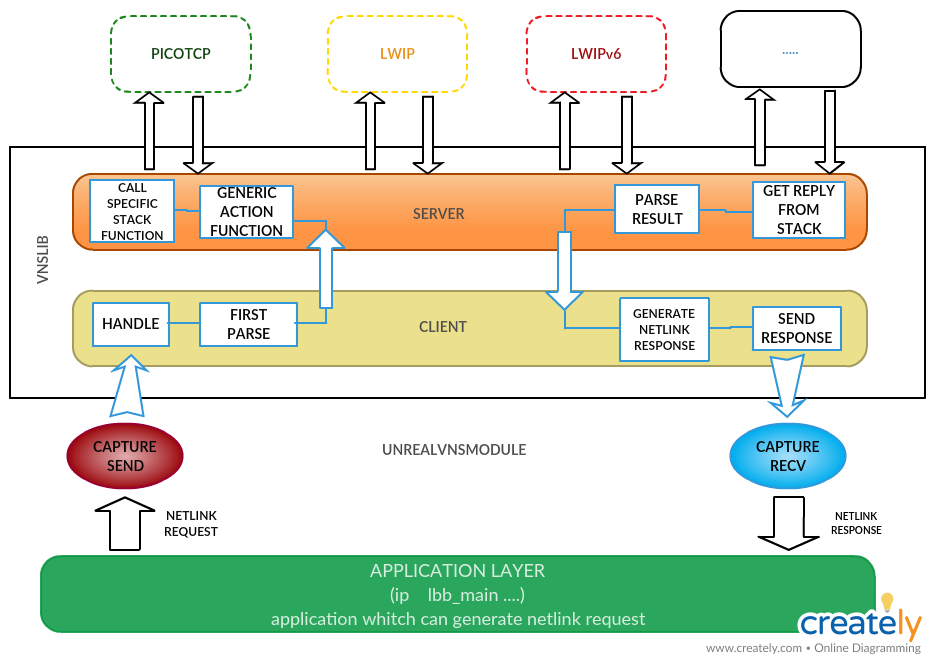
\includegraphics[width=15cm]{vnslib_scheme}%inserisce una figura larga 5cm
                                        %se si vuole usare va scommentata
%
%%%%%%%%%%%%%%%%%%%%%%%%%%%%%%%%%%%%%%%%%inserisce la legenda ed etichetta
                                        %   la figura con \label{fig:prima}
\caption[mappa concettuale libreria]{mappa concettuale libreria}\label{fig:map}
\end{center}
\end{figure}
\`E facile immaginare che la suddivisione riguardi l'interazione della libreria con l'utente.
\begin{description}                     %crea un elenco descrittivo
  \item[Client-side:] risiedono le funzioni che catturano i pacchetti netlink e che quindi permettono le configurazioni attraverso l'interfaccia netlink. In questa fase ci si occupa di fare parsing del pacchetto per costruire una struttura contenente i dati significativi.
  \item[Server-side:] back end della libreria, qui vengono gestiti i dati passati dal client per poi chiamare le specifiche funzioni approntate per configurare lo stack in uso.
\end{description}

\section{Moduli}
\section{Il Futuro}
%%%%%%%%%%%%%%%%%%%%%%%%%%%%%%%%%%%%%%%%%non numera l'ultima pagina sinistra
\clearpage{\pagestyle{empty}\cleardoublepage}

\chapter{Casi d'uso}                %crea il capitolo
%%%%%%%%%%%%%%%%%%%%%%%%%%%%%%%%%%%%%%%%%imposta l'intestazione di pagina
\lhead[\fancyplain{}{\bfseries\thepage}]{\fancyplain{}{\bfseries\rightmark}}
Di seguito alcuni esempi di utilizzo della libreria.
Le dimostrazioni seguenti sono state effettuate su una macchina con architettura amd64 e con installato il sistema operativo debian in versione sid (quindi unstable) ma sono state testate e riprodotteanche su altre configurazioni e distribuzioni GNU/Linux.

\section{Esempi}                 %crea la sezione

%%%%%%%%%%%%%%%%%%%%%%%%%%%%%%%%%%%%%%%%%non numera l'ultima pagina sinistra
\clearpage{\pagestyle{empty}\cleardoublepage}
%%%%%%%%%%%%%%%%%%%%%%%%%%%%%%%%%%%%%%%%%per fare le conclusioni


\chapter*{Conclusioni}
%%%%%%%%%%%%%%%%%%%%%%%%%%%%%%%%%%%%%%%%%imposta l'intestazione di pagina
\rhead[\fancyplain{}{\bfseries
CONCLUSIONI}]{\fancyplain{}{\bfseries\thepage}}
\lhead[\fancyplain{}{\bfseries\thepage}]{\fancyplain{}{\bfseries
CONCLUSIONI}}
%%%%%%%%%%%%%%%%%%%%%%%%%%%%%%%%%%%%%%%%%aggiunge la voce Conclusioni
                                        %   nell'indice
\addcontentsline{toc}{chapter}{Conclusioni} 
L'utilizzo di queste tipologie di stack dipende strettamente dalla diffusione del protocollo IPv6 e dei sistemi embedded e sembra essere la direzione in cui questo settore sta muovendosi.
La ricerca e lo sviluppo di questi meccanismi sono necessari ad ottenere un sistema performante e stabile quando IPv6 sar\`a l'ordinario, vanno poi considerati anche i vantaggi conseguenti nelle reti virtuali che gi\`a ora vengono utilizzate per la sperimentazione.

L'IoTh ne \`e un'astrazione pi\`u forte
In queste conclusioni voglio fare un riferimento alla
bibliografia: questo \`e il mio riferimento \cite{K3,K4}.
%%%%%%%%%%%%%%%%%%%%%%%%%%%%%%%%%%%%%%%%%imposta l'intestazione di pagina
\renewcommand{\chaptermark}[1]{\markright{\thechapter \ #1}{}}
\lhead[\fancyplain{}{\bfseries\thepage}]{\fancyplain{}{\bfseries\rightmark}}
\appendix                               %imposta le appendici
\chapter{Prima Appendice}               %crea l'appendice
In questa Appendice non si \`e utilizzato il comando:\\
%%%%%%%%%%%%%%%%%%%%%%%%%%%%%%%%%%%%%%%%%\verb"" � equivalente all'
                                        %   ambiente verbatim,
                                        %   ma si utilizza all'interno
                                        %   di un discorso.
\verb"\clearpage{\pagestyle{empty}\cleardoublepage}", ed infatti
l'ultima pagina 8 ha l'intestazione con il numero di pagina in
alto.
%%%%%%%%%%%%%%%%%%%%%%%%%%%%%%%%%%%%%%%%%imposta l'intestazione di pagina
\rhead[\fancyplain{}{\bfseries \thechapter \:Prima Appendice}]
{\fancyplain{}{\bfseries\thepage}}
\chapter{Seconda Appendice}             %crea l'appendice
%%%%%%%%%%%%%%%%%%%%%%%%%%%%%%%%%%%%%%%%%imposta l'intestazione di pagina
\rhead[\fancyplain{}{\bfseries \thechapter \:Seconda Appendice}]
{\fancyplain{}{\bfseries\thepage}}
\begin{thebibliography}{90}             %crea l'ambiente bibliografia
\rhead[\fancyplain{}{\bfseries \leftmark}]{\fancyplain{}{\bfseries
\thepage}}
%%%%%%%%%%%%%%%%%%%%%%%%%%%%%%%%%%%%%%%%%aggiunge la voce Bibliografia
                                        %   nell'indice
\addcontentsline{toc}{chapter}{Bibliografia}
%%%%%%%%%%%%%%%%%%%%%%%%%%%%%%%%%%%%%%%%%provare anche questo comando:
%%%%%%%%%%%\addcontentsline{toc}{chapter}{\numberline{}{Bibliografia}}
\bibitem{K1} Renzo Davoli. Internet of Threads. \url{http://www.cs.unibo.it/~renzo/papers/2013.iciw.pdf}, 2013.
\bibitem{K2} Renzo Davoli. Internet of Threads: Processes as Internet Nodes. \url{http://www.cs.unibo.it/~renzo/papers/2014.IntTechIoTh.pdf}, 2014.
\bibitem{K3} Renzo Davoli. Internet of Threads. \url{http://www.cs.unibo.it/~renzo/papers/ConfGARR11_SelectedPapers_Davoli.pdf}.
\bibitem{K4} Altran. picoTCP. \url{https://github.com/tass-belgium/picotcp}.
\bibitem{K5} Virtual Square Team. vuos. \url{https://github.com/virtualsquare/vuos}.
\bibitem{K6} Virtual Square Team. LWIPv6. \url{http://wiki.v2.cs.unibo.it/wiki/index.php/LWIPV6}.
\bibitem{K7} Virtual Square Team. UMview. \url{http://wiki.v2.cs.unibo.it/wiki/index.php/UMview}.
\bibitem{K8} Virtual Square Team. purelibc. \url{http://wiki.virtualsquare.org/wiki/index.php/PureLibc}.
\end{thebibliography}
%%%%%%%%%%%%%%%%%%%%%%%%%%%%%%%%%%%%%%%%%non numera l'ultima pagina sinistra
\clearpage{\pagestyle{empty}\cleardoublepage}
\chapter*{Ringraziamenti}
\thispagestyle{empty}
Qui possiamo ringraziare il mondo intero!!!!!!!!!!\\
Ovviamente solo se uno vuole, non \`e obbligatorio.
\end{document}








